\documentclass[11pt,letterpaper]{article}
%graph pour image H
\usepackage{float}

%Highlight
\usepackage{soul}

%Pour vecteur unitaire
\newcommand{\uvec}[1]{\boldsymbol{\hat{\textbf{#1}}}}

% Pour Dessin
\usepackage{tikz}
\usepackage{amsmath}
\usepackage{mathrsfs}
\usetikzlibrary{arrows.meta, positioning}

% Pour Braket de Quantique
\usepackage{braket}

% Pour circle red
\usetikzlibrary{shapes,
tikzmark}
\tikzset{every tikzmarknode/.style={%
draw=red, semithick, inner sep=2pt}
}


% Pour box paragraph
\usepackage{fancybox,framed}

% packetages pour ecrire en français
\usepackage[french]{babel}
\usepackage[utf8]{inputenc}
\usepackage[T1]{fontenc}

% pour les maths, les graphiques et la navigation dans le pdf
\usepackage{amsmath, amssymb, mathtools, mathrsfs, bm, array, units, amsthm, dsfont}
\usepackage{graphicx,caption,subcaption}
\graphicspath{{./}}
\usepackage{hyperref}
\hypersetup{
    pdftitle={Spectrométrie gamma avec un scintillateur NaI(Tl): identification d'isotopes, effet de la diffusion Compton et analyse du bruit de fond},
    pdfauthor={L-F. Brodeur (LFBRO1), S. L-Tremblay (SILAT10)}
}
\usepackage{physics} %très utile pour ecrire plus rapidement des matrices, des derivees, etc. Allez voir la documentation!

% marges, police de caractère et header
\usepackage{geometry}
\geometry{top=23mm, bottom=23mm, left=20mm, right=20mm}
\usepackage{cochineal}
\usepackage{fancyhdr}
\pagestyle{fancy}

\parindent=0mm % pas d'indentation

\lhead{L-F. Brodeur (IDUL: LFBRO1) et S. L-Tremblay (IDUL: SILAT10)}
\rhead{Détecteurs de radiations nucléaires}
\fancyheadoffset{0 cm}

\setlength{\headheight}{13.6pt}

% commandes pour ecrire des equations plus vite avec leur label
\newcommand{\beq}[1]{\begin{equation} \label{#1}}
\def\enq{\end{equation}}

% C'est parti!
\begin{document}
\shorthandoff{;:!?}
\thispagestyle{empty} % pas de header sur la première page
\begin{center}

\noindent
\begin{minipage}[t]{0.5\textwidth}
\raggedright
{\large GPH-3000 \textit{Travaux pratiques avancés}}\\
{\large Automne 2026 $\vert$ GPH-3000 (Groupe: 85213)}
\end{minipage}%
\begin{minipage}[t]{0.5\textwidth}
\raggedleft
{\large \textsc{L-F. Brodeur (IDUL: LFBRO1)}}\\
{\large \textsc{S. L-Tremblay (IDUL: SILAT10)}}
\end{minipage}
\\~\\
\vspace{1em}
{\Large \textbf{Spectrométrie gamma avec un scintillateur NaI(Tl):} } \\
{\Large \textbf{identification d'isotopes, effet de la diffusion Compton} } \\
{\Large \textbf{et analyse du bruit de fond} } \\[0.3em]
{\large Date du Laboratoire: 10 et 17 septembre 2026 \qquad\qquad\qquad Remis le \today}

\end{center}

\vspace{0.5em}
\subsection*{Résumé}
On ne le sent pas, mais des rayons gamma nous traversent en ce moment même: ils viennent du béton, des roches, et même de l'intérieur de notre propre corps. Cette expérience visait à étalonner un scintillateur NaI(Tl) couplé à un analyseur multicanaux (Easy-MCA-8k), à l'aide de cinq sources $\gamma$ connues (\textsuperscript{133}Ba, \textsuperscript{57}Co, \textsuperscript{60}Co, \textsuperscript{137}Cs, \textsuperscript{22}Na), puis à utiliser cet étalonnage pour identifier les sources qui forment le spectre du bruit de fond radioactif du laboratoire. Le modèle utilisé pour faire la correspondance entre les canaux de l'analyseur et l'énergie des rayons gamma a été un modèle quadratique ($R^2 = 0{,}99997$, RMSE $= 2{,}6~\text{keV}$), et la résolution du détecteur suit une loi de puissance $R = (122 \pm 29)\cdot E^{-0{,}44 \pm 0{,}04}~\%$, proche du comportement statistique attendu en $E^{-1/2}$. Sur le spectre du \textsuperscript{137}Cs, le front Compton et le pic de rétrodiffusion prédits par les mathématiques de la diffusion Compton (477,4~keV et 184,3~keV) correspondent, plus ou moins la résolution du détecteur, à ceux observés ($462 \pm 3$~keV et $201 \pm 3$~keV). Finalement, une acquisition de 36~minutes sans source a révélé un pic dominant à $1485 \pm 3~\text{keV}$, qui correspond à la raie de $1460{,}8~\text{keV}$ du \textsuperscript{40}K. Ceci indique que le potassium naturel, présent dans le béton, la brique et le sol, est la principale source de radioactivité ambiante du laboratoire. Ce même principe, combiné à une analyse de la direction des vents, a même permis à la centrale nucléaire de Forsmark, en Suède, de détecter la catastrophe de Tchernobyl deux jours après qu'elle a eu lieu \cite{forsmark}.

\section{Introduction}

Depuis la découverte de la radioactivité par Becquerel en 1896, on sait que certains noyaux se désintègrent et émettent des rayonnements pénétrants. Un compteur Geiger permet de détecter un rayon gamma, mais il ne donne aucune information sur son énergie. Un scintillateur par contre produit un signal dont l'amplitude est proportionnelle à l'énergie du photon incident, ce qui permet d'identifier l'isotope qui l'a émis en se désintégrant.

Il y avait deux objectifs à cette expérience. Premièrement, étalonner un scintillateur à l'iodure de sodium (NaI(Tl)) à l'aide de cinq sources $\gamma$ connues pour convertir les numéros de canal de l'analyseur en une énergie en keV. Deuxièmement, utiliser ce système calibré pour répondre à une question: quelles sont les sources de la radioactivité ambiante mesurée dans le laboratoire?

Certains mécanismes d'interaction des rayons gamma avec la matière sont premièrement présentés (Section~\ref{sec:theorie}). La procédure d'analyse est ensuite décrite (Section~\ref{sec:methodologie}). Les résultats généraux (Section~\ref{sec:resultats}) présentent l'étalonnage, la résolution du détecteur, l'anatomie du spectre du \textsuperscript{137}Cs (front Compton et pic de rétrodiffusion) et l'identification de la raie principale du bruit de fond. Ces résultats, leur qualité et leurs limites sont ensuite discutés (Section~\ref{sec:discussion}), et une conclusion (Section~\ref{sec:conclusion}) vient finalement clore le tout.

\section{Théorie}
\label{sec:theorie}

\subsection{Interaction des rayons gamma avec la matière}

Un rayon gamma qui traverse le cristal de NaI(Tl) peut y déposer son énergie de plusieurs façons \cite{knoll}. Sous $\sim$1~MeV, le régime qui nous concerne ici à l'exception des deux raies du \textsuperscript{60}Co, deux processus dominent:

\begin{itemize}
    \item L'effet photoélectrique: le photon cède toute son énergie à un électron du cristal, qui l'absorbe complètement. C'est ce processus qui produit le photopic, c'est-à-dire le pic étroit correspondant à l'énergie exacte du rayon gamma incident.
    \item La diffusion Compton: le photon ne cède qu'une partie de son énergie à un électron quasi libre et continue sa route, dévié, avec une énergie plus petite. L'énergie transférée à l'électron dépend de l'angle de diffusion $\theta$, qui varie entre $0^\circ$ (une diffusion vers l'avant) et $180^\circ$. C'est ce qui produit le continuum Compton, un plateau qui s'étend sous le photopic.
\end{itemize}

L'énergie maximale qu'un électron peut recevoir par diffusion Compton, correspondant à une rétrodiffusion à $180^\circ$, définit le front Compton:
\beq{eq:compton_edge}
    E_C = \frac{2E_\gamma^2}{m_e c^2 + 2E_\gamma} ,
\enq
où $E_\gamma$ est l'énergie du photon incident et $m_e c^2 = 511~\text{keV}$ l'énergie de masse au repos de l'électron. Au-delà de $E_C$, aucun événement Compton simple ne peut déposer plus d'énergie dans le cristal. C'est pourquoi le continuum chute rapidement à cette énergie.

Un second artefact, moins souvent discuté, est le pic de rétrodiffusion. Un photon peut se diffuser Compton à $180^\circ$ dans le blindage ou les matériaux environnant le détecteur (table, boîtier de la source, etc.) avant d'entrer dans le cristal, où il est alors absorbé par effet photoélectrique. L'énergie qu'il dépose correspond au complément de $E_C$:
\beq{eq:backscatter}
    E_{bs} = E_\gamma - E_C = \frac{E_\gamma}{1 + 2E_\gamma / (m_e c^2)} .
\enq
Ce pic apparaît donc sous forme d'une bosse dans le continuum, en dessous du front Compton.

\subsection{Radioactivité ambiante}

Même en l'absence de toute source radioactive volontaire, un détecteur $\gamma$ enregistre toujours un signal. Ce bruit de fond provient à la fois du rayonnement cosmique et de la radioactivité naturelle présente dans notre environnement immédiat: les matériaux de construction (béton, brique, granite) contiennent des traces d'éléments radioactifs à longue durée de vie, principalement le \textsuperscript{40}K et les descendants des chaînes de désintégration de l'\textsuperscript{238}U et du \textsuperscript{232}Th \cite{unscear}. Le \textsuperscript{40}K est particulièrement intéressant: il représente environ 0,012~\% du potassium naturel, a une demi-vie de 1,25 milliard d'années, et se désintègre 11~\% du temps par capture électronique vers un état excité du \textsuperscript{40}Ar qui se désexcite et émet un photon $\gamma$ à 1460,8~keV \cite{nndc}. Comme le potassium est abondant dans le corps humain, les os et les matériaux de construction, cette raie est presque toujours la signature dominante du bruit de fond ambiant dans un laboratoire.

\section{Méthodologie}
\label{sec:methodologie}

\subsubsection*{Étalonnage}
Cinq sources scellées (\textsuperscript{133}Ba, \textsuperscript{57}Co, \textsuperscript{60}Co, \textsuperscript{137}Cs, \textsuperscript{22}Na) ont été mesurées selon le protocole \cite{protocole}, fournissant onze raies $\gamma$ de référence entre 30,85~keV et 1332,50~keV (Tableau~\ref{tab:acquisitions}). Chaque source a été placée devant le détecteur pour un temps d'acquisition suffisant pour obtenir un photopic net (de 3 à 15~minutes selon l'activité de la source), tandis qu'une acquisition beaucoup plus longue (36~minutes) a été faite sans aucune source, pour caractériser le bruit de fond.

\subsubsection*{Analyse}
L'ensemble du traitement a été fait en Python. Pour chaque raie de référence, la région du spectre autour du canal attendu est analysée pour trouver un maximum local de comptes. Les onze couples (canal, énergie) sont ensuite utilisés pour ajuster une relation d'étalonnage $E(\text{canal})$ quadratique. Tous les spectres présentés plus bas sont en taux de comptage (coups/s), obtenus en divisant le nombre de comptes par le temps vif (live time) fourni par le logiciel d'acquisition. Le temps vif exclut les intervalles où l'électronique était occupée à traiter une impulsion précédente, ce qui corrige donc pour le temps mort. Le taux de comptage du bruit de fond est aussi soustrait de chaque spectre de source, pour isoler le signal de la source elle-même.

Les incertitudes sont propagées par dérivées partielles. Une énergie obtenue à partir d'un pic à $\mu \pm \Delta\mu$ (où $\Delta\mu$ vient de la matrice de covariance du curve fit) et de l'étalonnage $E = a\,\mu^2 + b\,\mu + c$ (éq.~\ref{eq:calib}) a pour incertitude
\beq{eq:dE}
    \Delta E = \left|\frac{\partial E}{\partial \mu}\right| \Delta\mu = \left(2a\mu + b\right) \Delta\mu .
\enq

\begin{table}[htbp]
\centering
\caption{Sources utilisées, raies de référence et statistiques d'acquisition. Le temps vif (utilisé pour normaliser les spectres en taux de comptage) et le temps réel sont donnés ensemble avec la fraction de temps mort qu'ils impliquent.}
\label{tab:acquisitions}
\small
\begin{tabular}{lcc}
\hline
Source & Raies utilisées (keV) & Temps vif / réel (s), temps mort \\
\hline
\textsuperscript{133}Ba & 30,85 / 81,00 / 302,85 / 356,02 & 372 / 383~s (2,9~\%) \\
\textsuperscript{57}Co  & 122,06 & 675 / 687~s (1,7~\%) \\
\textsuperscript{60}Co  & 1173,20 / 1332,50 & 896 / 909~s (1,4~\%) \\
\textsuperscript{137}Cs & 32,00\textsuperscript{a} / 661,70 & 180 / 232~s (22,4~\%) \\
\textsuperscript{22}Na  & 511,00 / 1274,50 & 186 / 196~s (5,1~\%) \\
Bruit de fond & aucune (identification a posteriori) & 2155 / 2157~s (0,1~\%) \\
\hline
\end{tabular}
\\[0.3em]
{\footnotesize \textsuperscript{a} Raie X caractéristique du baryum (transition K), et non une désexcitation nucléaire du \textsuperscript{137}Cs lui-même.}
\end{table}

\section{Résultats}
\label{sec:resultats}

\subsection{Étalonnage et résolution en énergie}

La Figure~\ref{fig:calib} montre les onze points d'étalonnage ainsi que le modèle quadratique,
\beq{eq:calib}
    E(\text{canal}) = a\,\text{canal}^2 + b\,\text{canal} + c ,
\enq
avec $a = (4{,}5 \pm 1{,}0) \times 10^{-6}~\text{keV}$, $b = (0{,}390 \pm 0{,}003)~\text{keV}$ et $c = (-3{,}0 \pm 1{,}9)~\text{keV}$ (incertitudes tirées de la matrice de covariance du curve fit). Ce modèle donne $R^2 = 0{,}99997$ et une erreur quadratique moyenne (RMSE) de $2{,}6~\text{keV}$.

La résolution relative $R = \text{FWHM}/E$ de chaque photopic (Tableau~\ref{tab:peaks}), tracée à la Figure~\ref{fig:resolution}, diminue avec l'énergie. Un ajustement linéaire de $\ln R$ en fonction de $\ln E$ donne la relation
\beq{eq:resolution}
    R(E) = (122 \pm 29) \cdot E^{-0{,}44 \pm 0{,}04}~\% \quad (E \text{ en keV}) ,
\enq
proche de la dépendance $E^{-1/2}$ attendue pour un détecteur limité par la statistique de comptage des photons de scintillation \cite{knoll}. Les incertitudes viennent de la matrice de covariance du curve fit.

\begin{table}[htbp]
\centering
\caption{Détail des onze raies d'étalonnage: énergie de référence, numéro de canal du pic et résolution en énergie ($R = \text{FWHM}/E_{\text{lit.}}$).}
\label{tab:peaks}
\footnotesize
\renewcommand{\arraystretch}{0.85}
\begin{tabular}{lcccc}
\hline
Source & $E_{\text{lit.}}$ (keV) & Canal & FWHM (keV) & $R$ (\%) \\
\hline
\textsuperscript{133}Ba & 30,85  & 82   & 8,0  & 26,1 \\
\textsuperscript{133}Ba & 81,00  & 221  & 12,6 & 15,6 \\
\textsuperscript{133}Ba & 302,85 & 781  & 25,6 & 8,4  \\
\textsuperscript{133}Ba & 356,02 & 921  & 42,1 & 11,8 \\
\textsuperscript{57}Co  & 122,06 & 319  & 16,2 & 13,3 \\
\textsuperscript{60}Co  & 1173,20& 2910 & 61,6 & 5,2  \\
\textsuperscript{60}Co  & 1332,50& 3296 & 66,8 & 5,0  \\
\textsuperscript{137}Cs & 32,00  & 83   & 9,9  & 31,0 \\
\textsuperscript{137}Cs & 661,70 & 1659 & 57,8 & 8,7  \\
\textsuperscript{22}Na  & 511,00 & 1300 & 54,5 & 10,7 \\
\textsuperscript{22}Na  & 1274,50& 3166 & 57,9 & 4,5  \\
\hline
\end{tabular}
\renewcommand{\arraystretch}{1}
\end{table}

\begin{figure}[htbp]
    \centering
    
\includegraphics[width=\textwidth]{../figures/01_calibration.png}
    \caption{Énergie en fonction du numéro de canal pour les onze raies.}
    \label{fig:calib}
\end{figure}

\begin{figure}[htbp]
    \centering
    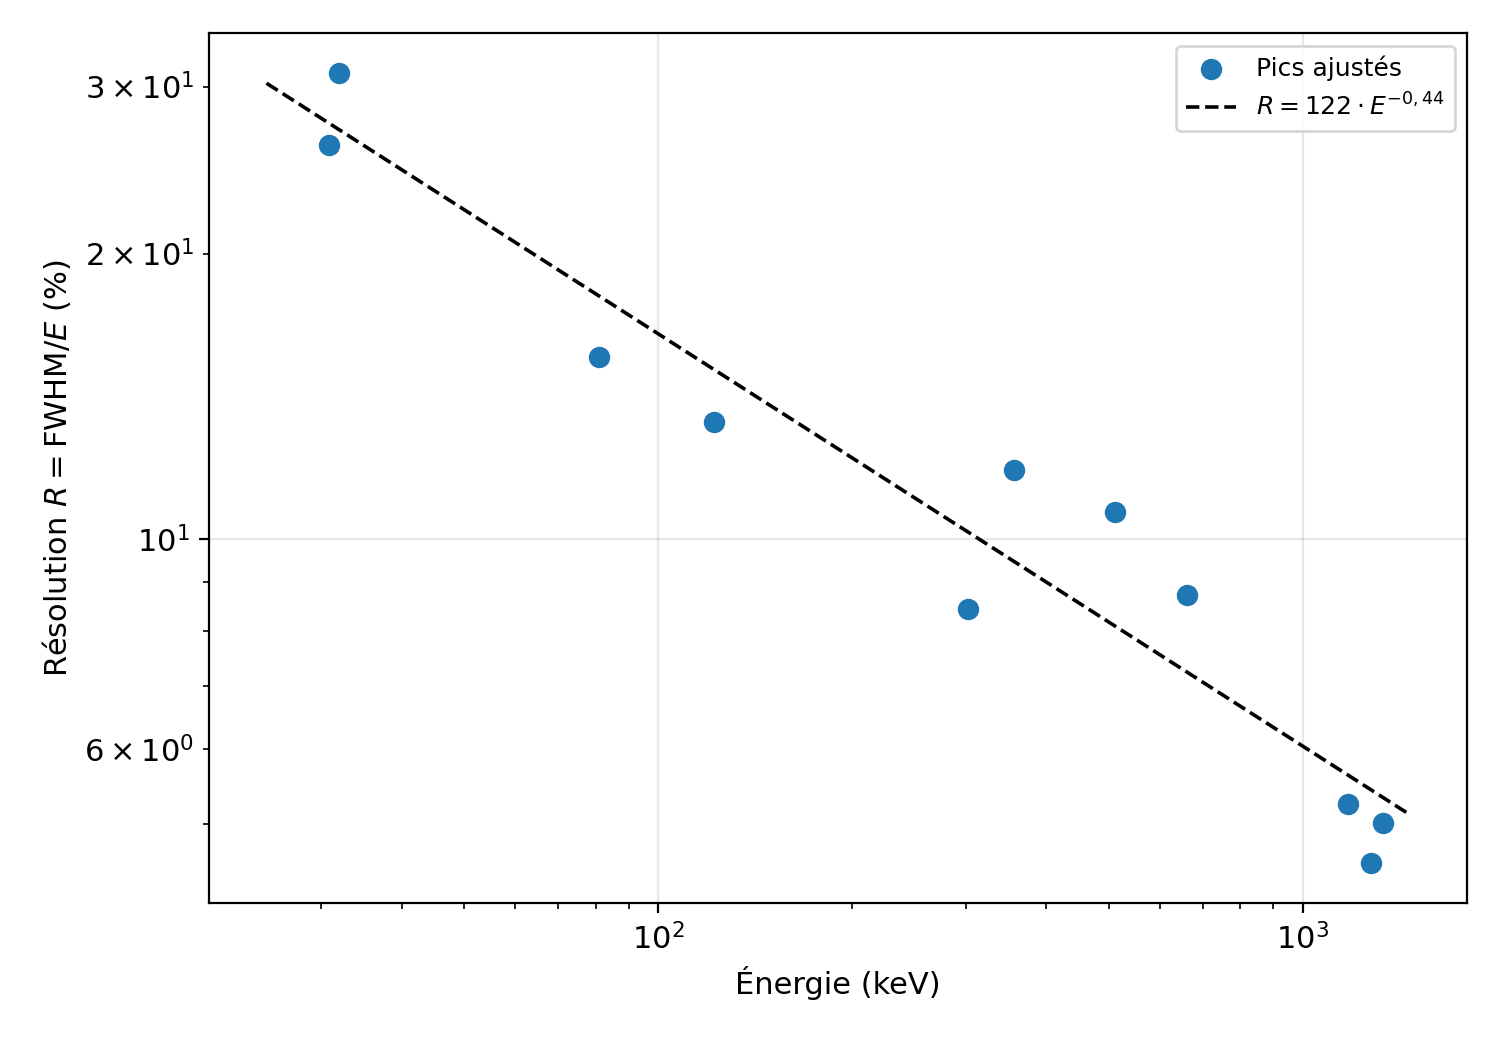
\includegraphics[width=\textwidth]{../figures/10_resolution.png}
    \caption{Résolution versus énergie pour les onze photopics. L'exposant de $-0{,}44$ est proche du $-0{,}5$ attendu.}
    \label{fig:resolution}
\end{figure}

\subsection{Anatomie d'un spectre: effet photoélectrique, diffusion Compton et rétrodiffusion}
\label{sec:anatomie}

Le spectre du \textsuperscript{137}Cs (Figure~\ref{fig:compton}) est intéressant parce que la source n'émet qu'une seule raie $\gamma$ (661,7~keV): toutes les structures observées avant le photopic proviennent donc de la physique de l'interaction gamma avec la matière. On y voit:
\begin{itemize}
    \item le photopic à 661,7~keV (effet photoélectrique, Tableau~\ref{tab:peaks}).
    \item un plateau Compton entre $\sim 50$ et $\sim 430$~keV, relativement plat comme attendu pour une diffusion à petit angle sur des électrons quasi libres.
    \item une chute abrupte du continuum, dont le point à mi-hauteur entre le plateau et le creux ($462 \pm 3~\text{keV}$) est proche du front Compton théorique (éq.~\ref{eq:compton_edge}, $477{,}4~\text{keV}$).
    \item une bosse de rétrodiffusion, dont le centre est à $201 \pm 3~\text{keV}$, un peu au-dessus de la prédiction de $184{,}3~\text{keV}$ (éq.~\ref{eq:backscatter}).
    \item un pic mesuré à 29,5~keV qui est la raie X caractéristique du baryum (produit de désintégration du \textsuperscript{137}Cs), émise lors du réarrangement électronique qui suit la désexcitation nucléaire. Sa valeur théorique est de 32,0~keV \cite{nndc}.
\end{itemize}

\begin{figure}[htbp]
    \centering
    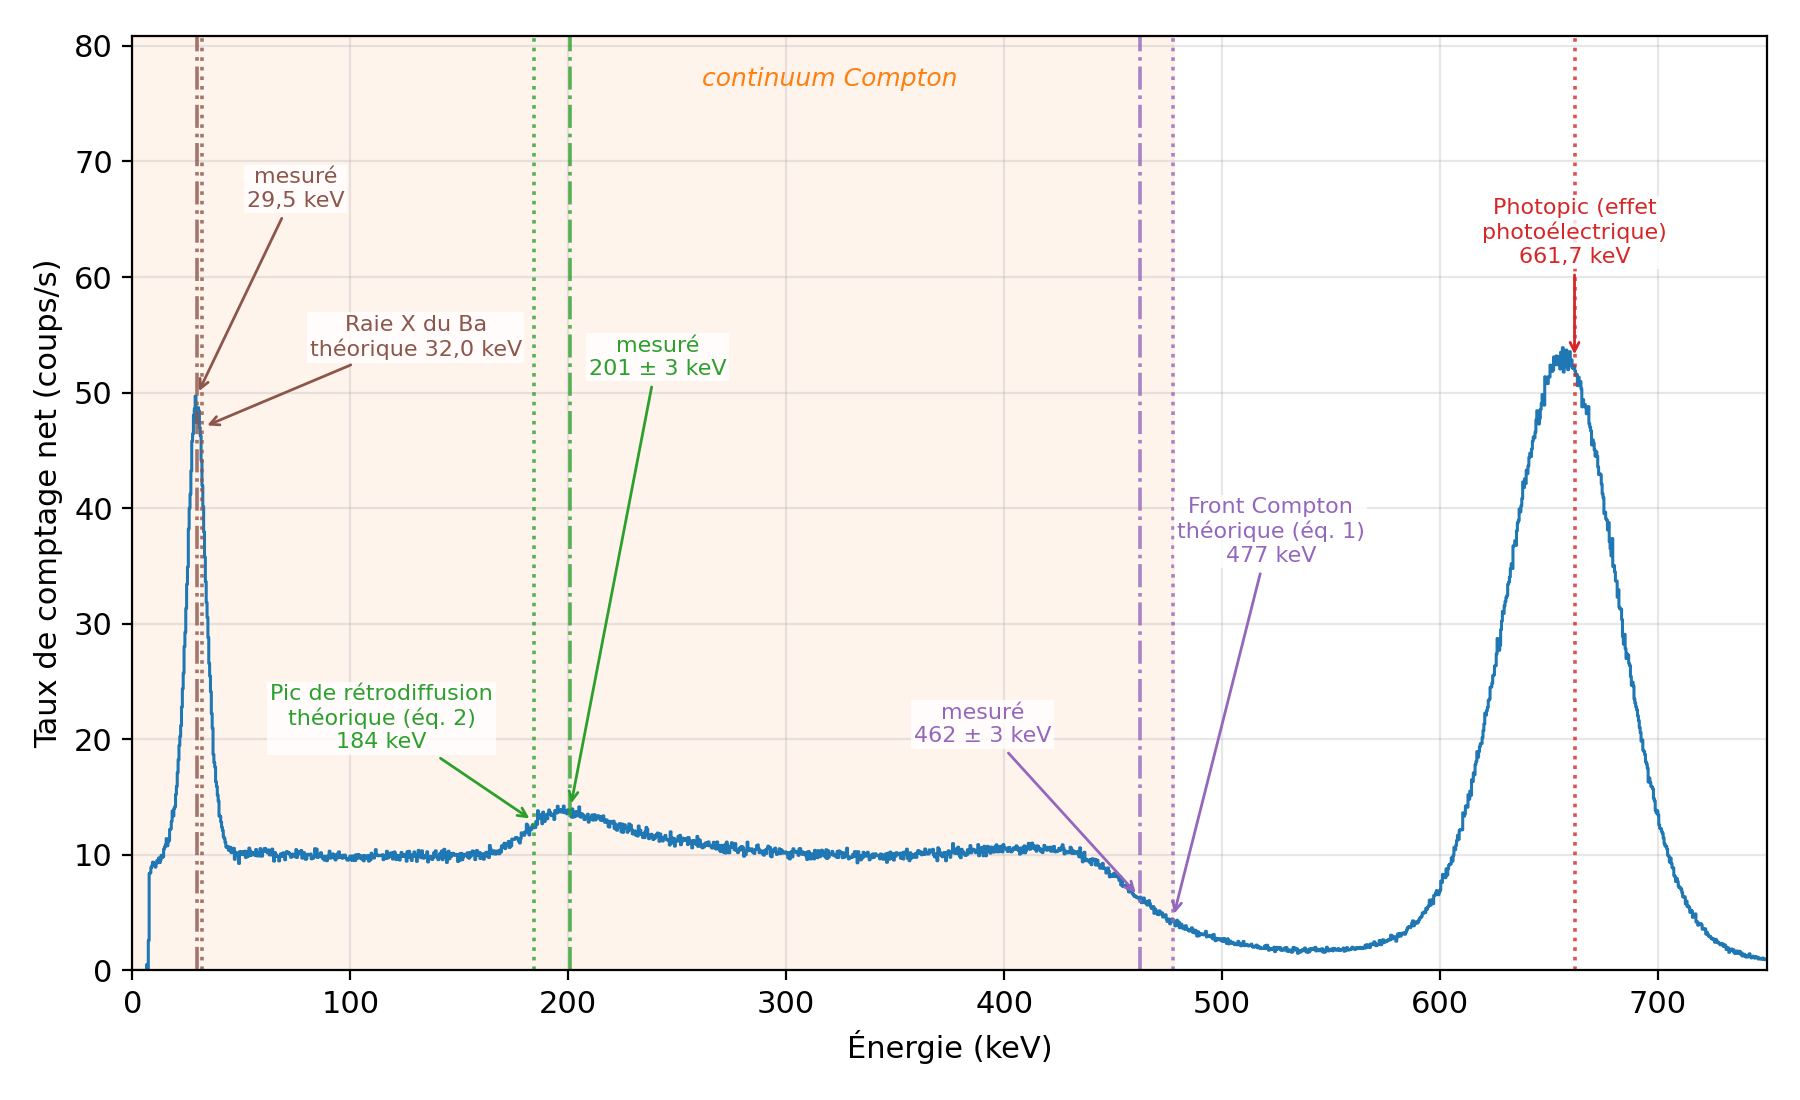
\includegraphics[width=0.74\textwidth]{../figures/09_compton_cs137.png}
    \caption{Spectre du \textsuperscript{137}Cs: les lignes pointillées courtes marquent les positions théoriques du front Compton, du pic de rétrodiffusion (éq.~\ref{eq:compton_edge},~\ref{eq:backscatter}) et de la raie X du baryum, les lignes mixtes marquent leurs positions mesurées sur le spectre. La zone orange délimite le continuum Compton.}
    \label{fig:compton}
\end{figure}

\subsection{Identification du bruit de fond ambiant}

Le spectre du bruit de fond (Figure~\ref{fig:background}), accumulé sur 36~minutes en l'absence de toute source, montre une tendance qui décroît avec l'énergie. Un ajustement gaussien de la structure entre $\sim 1350$ et $\sim 1550$~keV situe son centroïde à $1485 \pm 3~\text{keV}$, similaire à la raie de référence du \textsuperscript{40}K à $1460{,}8~\text{keV}$ \cite{nndc}.

\begin{figure}[htbp]
    \centering
    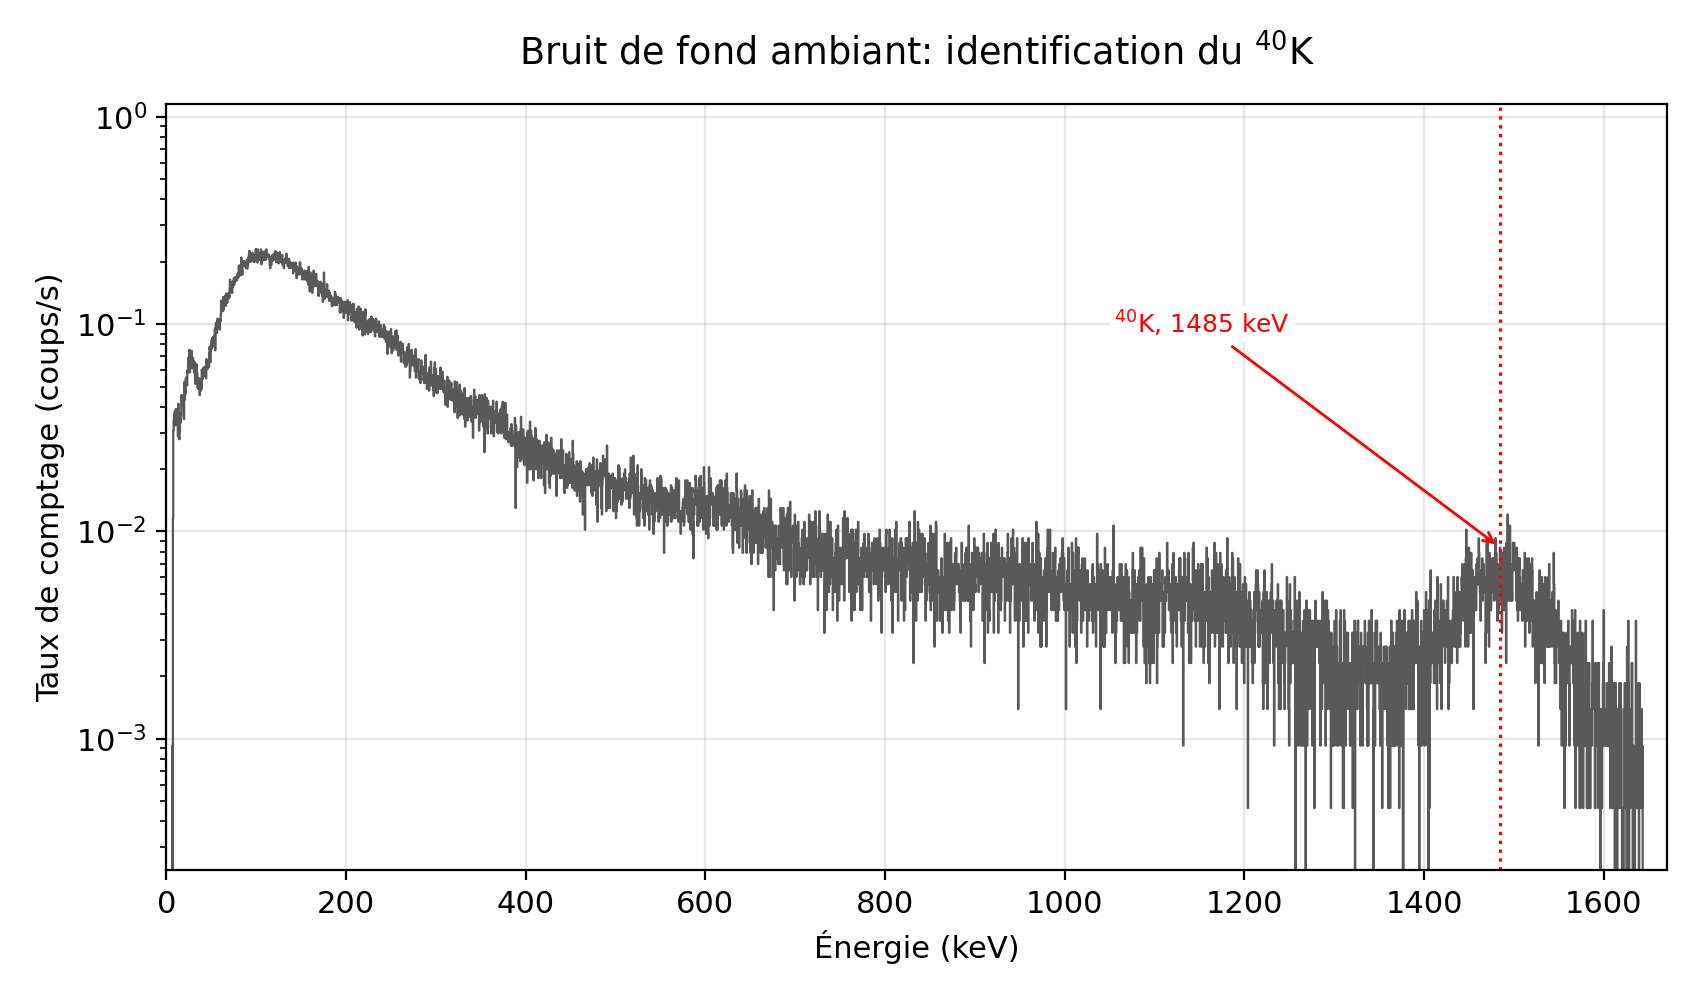
\includegraphics[width=0.68\textwidth]{../figures/08_background_K40.png}
    \caption{Spectre du bruit de fond ambiant. La raie identifiée à $1485 \pm 3~\text{keV}$ est attribuée au \textsuperscript{40}K (1460,8~keV), présent naturellement dans le béton, le sol et le corps humain.}
    \label{fig:background}
\end{figure}

\section{Discussion}
\label{sec:discussion}

\subsubsection*{Qualité de l'étalonnage}
Le modèle quadratique est un bon choix pour l'étalonnage. Avec $R^2 = 0{,}99997$ et un RMSE de 2,6~keV sur onze raies entre 30~keV et 1,33~MeV, il reproduit très bien les énergies de référence.

\subsubsection*{Front Compton et rétrodiffusion}
Les positions mesurées (Section~\ref{sec:anatomie}) diffèrent des prédictions de 15~keV pour le front et de 17~keV pour la rétrodiffusion. C'est moins que la largeur des pics à ces énergies (FWHM d'environ 39~keV à 462~keV et 24~keV à 201~keV, d'après l'équation~\ref{eq:resolution}), donc ces résultats appuient les mathématiques de la diffusion Compton. Le front mesuré est plus bas que prévu, ce qui s'explique probablement par la méthode utilisée pour trouver la position du front (point à mi-hauteur). Le pic de rétrodiffusion est plus haut que prévu parce que l'équation~\ref{eq:backscatter} suppose un angle de exactement $180^\circ$. Les photons diffusés à des angles un peu plus petits dans les matériaux autour du détecteur arrivent avec une énergie un peu plus grande, ce qui déplace le centre de la bosse vers le haut.

\subsubsection*{Identification du \textsuperscript{40}K}
L'écart entre la valeur mesurée ($1485 \pm 3~\text{keV}$) et la valeur de référence ($1460{,}8~\text{keV}$) est de $24~\text{keV}$, c'est sept fois l'incertitude sur le centroïde (éq.~\ref{eq:dE}). Cet écart est donc significatif, et il est aussi beaucoup plus grand que celui des raies d'étalonnage. La cause la plus probable de l'écart est que $1461~\text{keV}$ se situe au-delà de la raie d'étalonnage la plus énergétique (1332,5~keV, \textsuperscript{60}Co), donc le modèle extrapole hors de son domaine. Le reste de l'écart pourrait venir du bruit de fond sous le pic, qui décroît beaucoup dans cette région.

\subsubsection*{Limites et améliorations}
Le montage utilisé ne permet pas de mesurer une activité absolue, car nous n'avons aucune information sur la distance source-détecteur. Une prochaine expérience pourrait prendre en compte la géométrie source-détecteur à chaque manipulation, ce qui permettrait de faire une estimation de l'activité des sources. Aussi, une source d'étalonnage au-dessus de 1332,5~keV permettrait de réaliser un meilleur étalonnage.

\section{Conclusion}
\label{sec:conclusion}

Le scintillateur NaI(Tl) a été étalonné avec succès à l'aide de cinq sources $\gamma$ connues. Le modèle utilisé pour convertir les canaux en énergie a été un modèle quadratique, avec une précision de 2,6~keV (RMSE) sur une plage de 30~keV à 1,33~MeV. Les deux objectifs de l'expérience ont été atteints: l'instrument calibré a permis de vérifier la physique de la diffusion Compton et d'identifier le \textsuperscript{40}K comme principale source du bruit de fond ambiant du laboratoire. L'énergie mesurée pour ce pic ($1485 \pm 3~\text{keV}$) est toutefois 24~keV au-dessus de la valeur de référence, un écart qui vient probablement de l'extrapolation de l'étalonnage au-delà de 1332,5~keV. Aussi, la résolution en énergie du détecteur a été caractérisée sur toute la plage, ce qui a montré un comportement proche du comportement théorique ($R \propto E^{-0{,}44}$, contre $E^{-0{,}5}$ attendu).

\renewcommand{\refname}{Bibliographie}
\begin{thebibliography}{9}

\bibitem{knoll}
Knoll, G.F. \textit{Radiation Detection and Measurement}, 4\textsuperscript{e} édition. John Wiley \& Sons, 2010.

\bibitem{nndc}
National Nuclear Data Center, Brookhaven National Laboratory. \textit{NuDat 3.0: Nuclear Structure and Decay Data}. \url{https://www.nndc.bnl.gov/nudat3/} (données du \textsuperscript{40}K, \textsuperscript{133}Ba, \textsuperscript{57}Co, \textsuperscript{60}Co, \textsuperscript{137}Cs, \textsuperscript{22}Na).

\bibitem{protocole}
Département de physique, de génie physique et d'optique, Université Laval. \textit{GPH-3000, Travaux pratiques avancés: Détecteurs de radiations nucléaires}, version 2019-09-23, et \textit{Résumé des manipulations}, version 2022-09-22.

\bibitem{unscear}
United Nations Scientific Committee on the Effects of Atomic Radiation (UNSCEAR). \textit{Sources and Effects of Ionizing Radiation: UNSCEAR 2000 Report to the General Assembly, with Scientific Annexes, Volume I: Sources}. United Nations, New York, 2000.

\bibitem{forsmark}
Wikipédia. \textit{Centrale nucléaire de Forsmark}, section « Découverte de la catastrophe de Tchernobyl ». \url{https://fr.wikipedia.org/wiki/Centrale_nucl\%C3\%A9aire_de_Forsmark#D\%C3\%A9couverte_de_la_catastrophe_de_Tchernobyl} (consulté en septembre 2026).

\end{thebibliography}

\section*{Annexe A: spectres individuels des sources d'étalonnage}

Les quatre figures suivantes montrent les spectres complets des sources utilisées pour l'étalonnage (à l'exception du \textsuperscript{137}Cs, présenté en détail à la Figure~\ref{fig:compton}), avec les raies de référence identifiées.

\begin{figure}[H]
    \centering
    
\includegraphics[width=0.72\textwidth]{../figures/02_spectre_Ba133.png}
    \caption{Spectre du \textsuperscript{133}Ba, quatre raies de référence de 30,85 à 356,02~keV.}
\end{figure}

\begin{figure}[H]
    \centering
    
\includegraphics[width=0.72\textwidth]{../figures/03_spectre_Co57.png}
    \caption{Spectre du \textsuperscript{57}Co, raie unique à 122,06~keV.}
\end{figure}

\begin{figure}[H]
    \centering
    
\includegraphics[width=0.72\textwidth]{../figures/04_spectre_Co60.png}
    \caption{Spectre du \textsuperscript{60}Co, doublet caractéristique à 1173,20 et 1332,50~keV.}
\end{figure}

\begin{figure}[H]
    \centering
    
\includegraphics[width=0.72\textwidth]{../figures/06_spectre_Na22.png}
    \caption{Spectre du \textsuperscript{22}Na, incluant le pic d'annihilation à 511,00~keV et la raie nucléaire à 1274,50~keV.}
\end{figure}

\end{document}
